\newcommand{\op}{\operatorname}
\newcommand{\ind}{\stackrel{ind.}{\sim}}
\section{Introduction}
Profiling gene expression is common problem in modern biology. It is also a classic $n \ll p$ example, inspiring statistical advances in multiple testing. Because the presence of a meaningful biological effect fits awkwardly into the NHST framework, arguably most questions of interest are better addressed through estimation \citet{deseq2014}. This is the approach that we pursue here.

% Current estimation methodologies can be understood as improving upon a ``straight" estimator by modeling gene-specific model parameters to borrow information across genes. \textit{Insert analogy to Stein's estimator}.

Because there are many genes to observe, a gene expression experiment presents an opportunity to learn the underlying distribution of the gene-specific parameters, $\mathcal{P}$. Given that gene profiling studies typically measure expression of tens of thousands of genes, there is substantial information to estimate $\mathcal{P}$. If we assume a standard parameteric family form for $\mathcal{P}$, then we should be able to estimate $\mathcal{P}$ precisely.
% The advantages of such hierarchical models have been shown to work well in practice, regardless of whether the distributional form of the random effects restrict should be assumed to have a simple form, will tend to be estimated very precisely. If the model is overly simplistic, the information borrowed across genes will tend to be quite vague. 
A benefit of hierarchical modeling is to regularize estimation for gene-specific parameters by shrinking the posterior distribution of these parameters toward the mass of their distribution. Regularization through the use of `shrinkage priors', or equivalent methods, has proven to be a useful tool even when the distributional form is misspecified.

Because of its essential role, the shape of the tail, vis a vis the choice of the hierarchical model, should be considered. We showed that the choice affected the number of genes called as well as which ones.

\citet*{lithio} considered reparameterizing the linear predictors to minimize the correlations of the gene-specific effects, in part to motivate the use of independent prior distributions. They find that the parameterization has a significant impact on the performance of the model. We hope avoid such sensitivities through the use of a nonparametric prior on these parameters.

In \citet{voom}, the authors proposed using a nonparametric estimate of the mean variance relationship using the straight estimates as data to produce precision estimates for each datum, thereby borrowing information about the measure of uncertainty within a gene. In Niemi et al, 2016, the authors used an empirical Bayes approach that considered the marginal empirical distributions of the straight estimators to inform the selection of prior distributions of the regression coefficients.

\citet{liu} proposed a semiparametric model for differential expression. In their model, a gamma mixture of Poisson was used and information was borrowed across genes only for the log-fold-change parameter, which was given a Dirichlet process prior.

In the present article, we propose a Bayesian nonparametric model which extends the approach taken in \citet{liu} by modeling the joint distribution of all gene-specific parameters with a Dirichlet process. The goal of this work is to provide a method that increases the amount of information being borrowed across genes and is insensitive to the choice of parameterization.


\section{RNA-seq gene expression data}
\label{sec:data}
The starting point for our analyses is an array of RNA-seq total reads for $N$ samples, aligned to $G$ genes. For details on preprocessing, see (Nettleton and Datta?) 

\subsection{Normalization and weighting}
\paragraph{Normalization}


\paragraph{voom}
Theory suggests that an RNA-seq count, $C$, would have a Poisson distribution, with variance equal to the mean ($\op{V}(C|\mu)=\mu, \mu=\op{E}(C)$), if the RNA from the same sample were sequenced repeatedly. Biological variation (either between subjects or through repeated sampling) leads overdispersion of the counts. Often, the negative binomial distribution is used because its variance is quadratic with the mean ($\op{V}(C|\mu)=\mu+\phi\mu^2$). Because gene expression is usually measured on the log scale, through an application of the delta method, we can re-express this approximately in terms of the log-count ($\op{V}(\log C|\mu) \approx \frac{1}{\mu} + \phi$. While this assumption may be adequate for genes with similar expression levels, empirical studies suggest that the overdispersion parameter, $\phi$, tends to be larger for genes with lower expression than those with higher expression.

\cite{voom} proposed \textit{voom}, a way to incorporate between-gene information about the mean-variance relationship in an RNA-seq data set through precision weighting of individual log-counts, making the data amenable to analysis with a linear model. It works by first calculating, for each gene, a sample standard deviation and mean log-count, and then fitting a LOWESS curve, treating the square root standard deviation as a response and the mean log-count as the predictor. Fitted values are then calculated for all counts, which are converted into precision weights.

Rather than assuming the mean-variance relationship of the negative binomial and allowing for an adjustment of the degree of overdispersion from gene to gene, voom's precision weighting scheme estimates the mean-variance relationship from the data and assumes that it applies both within as well as across genes. We use the precision weights as an input to our model (Section \ref{sec:model}) which estimates a gene-specific variance parameter. Our use of voom in our pipeline implies a gene-specific mean-variance relationship \textit{for the log counts} given by
$$\op{V}(\log C|\mu)=\sigma^2_g \widehat{\op{V}_{voom}(\log C|\mu)}.$$


\subsection{Maize data of Paschold et al.}


\section{Bayesian nonparametric model}
When the model assumptions on $\mathcal{P}$ restrict the posterior for $\mathcal{P}$ to a set that cannot realistically represent $\mathcal{P}$, this limits the efficiency of the hierarchical model. To illustrate, suppose we observe $y_{gn},\; g=1,\ldots,100,\;n=1,\ldots 1$, and we can reasonably assume that $y_{gn}|\mu_g \ind \op{N}(\mu_g,\sigma^2)$, i.e. the data are conditionally normal, with a constant error variance. Suppose we 

\label{sec:model}
Let $y_{gn}$ represent the observed expression (possibly after transformation) for gene $g$, sample $n$. Let $x_{n}^\top$ be the row of the design matrix $X$ corresponding to sample $n$. We will use the upper case letters $G$ and $N$, to denote the number of genes and samples, respectively. To accommodate observation-level weights, $w_{gn}$, which provide a correction for a global mean-variance relationship in the data. For the observed data, we assume the data model
\begin{equation}
y_{gn} \sim \op{N} \left( x_{n}^\top \beta_g, \frac{\sigma^2_g}{w_{gn}} \right).
\end{equation}
Next, we propose to model jointly

\begin{equation}
\left(\beta_g^\top,\sigma^2_g\right) \ind \mathcal{P},
\end{equation}
where we specify a Dirichlet process on $\mathcal{P}$, i.e.,

\begin{equation}
\mathcal{P} \sim \op{DP}(\alpha \mbox{Q}).
\end{equation}

\iftoggle{thesis}{
The use of this prior, due to \citet{ferguson}, is a distribution over probability distributions, such that for any finite disjoint partition $\{A_i\}_{i>=1}^n$ on $\mathbb{R}^p$, $\mathcal{P}$ is a random measure such that the joint distribution $\left(\mathcal{P}(A_1),\ldots,\mathcal{P}(A_n)\right) \sim \op{Dir}\left(\alpha Q(A_1),\ldots,\alpha Q(A_n)\right).$ The Dirichlet process has two parameters: $Q$, the base measure, represents a prior guess at the distribution. $\alpha$, the concentration parameter expresses the degree to which $\mathcal{P}$ will agree with $Q$ on any set $A$. This follows from the definition given above and known properties of the Dirichlet distribution, i.e., $\op{E}\left(\mathcal{P}(A)\right)=Q(A)$, and $\op{V}\left(\mathcal{P}(A)\right)=\frac{Q(A)(1 - Q(A)}{\alpha + 1}$, showing that $\mathcal{P}(A) \stackrel{p}{\rightarrow} Q(A)$ as $\alpha \rightarrow \infty$ for any set $A$. 
}{}
By modeling $\mathcal{P}$ with a Dirichlet process one can be noninformative about the overall shape of $\mathcal{P}$, allowing for irregular shapes, multimodality, and so forth. An argument can be made that by incorporating our uncertainty about these features of the distribution is required for coherent interpretation of the posterior distribution \citep{walker2010bayesian}. For more information about the properties of the DP, see \cite{ferguson}.

As shown by \citet{sethuraman}, it follows from the definition of the Dirichlet process that $\mathcal{P}$ is almost surely discrete and realizations of $\mathcal{P}$ can be produced by the following stick-breaking construction:

Let 
\begin{equation}
\mathcal{P} =\sum_{k=1}^\infty \pi_k \delta_{\left(\tilde{\beta}_k^\top ,\tilde{\sigma}^2_k\right)}.
\end{equation}
Here $\delta_{(.)}$ is the Dirac delta function. Note that although almost sure discreteness is a property applicable to ``draws'' from a DP, the posterior for $\mathcal{P}$ is in fact a mixture of DP \citep{antoniak}. An implication of discretness can be thought of as a ``bet on sparsity"; that there are actually a finite (but unspecified) number of unique values that $(\beta_g^\top,\sigma^2_g)$ can take.  
 The ``atoms" distributed according to $Q$, specified by the product measure

\begin{equation}
\tilde{\beta}_k \sim \op{N}(m_\beta, C_\beta),\quad \tilde{\sigma}^2_k \sim \op{IG}(a_{\sigma^2}, b_{\sigma^2}).
\end{equation}

``$\op{IG}(a,b)$" refers to the inverse gamma distribution which we parameterize by shape and scale parameters, $a$ and $b$ with density given by
\begin{equation*}
p(x|a,b) = \frac{b^a}{\Gamma(a)}x^{a+1}e^{-b/x}.
\end{equation*}


The mixture weights, $\pi_k$,  follow a stick-breaking process \cite{sethuraman}. Using the reparameterization,

\begin{equation}
\nu_k = \frac{\pi_k}{1 - \sum_{l=1}^{k-1} \pi_l},
\end{equation}

$\nu_k$ representing a proportion of the total probability remaining after $k-1$ breaks. For the stick-breaking construction of the DP, the $\nu_k$ are modeled by:
\begin{equation}
\nu_k \ind \op{Beta}(1, \alpha).
\end{equation}

This assumption induces a stochastically decreasing ordering of the weights. Additionally, note that $\sum_{k=1}^K \pi_k \stackrel{p}{\rightarrow} 1$ as $K\rightarrow \infty$. 

\section{Simulation study 1}
Since the proposed BNP method uses voom weights, we did a simulation study to compare the our method to the voom-limma method for RNA-seq data. The voom-limma method fits a linear model to the data under the same transformation conditional on the same voom quality weights, but proceeds by fitting each gene independently. Thus, a comparison of the estimates obtained under BNP model to the voom-limma estimates will show the result of borrowing information across genes via the Dirichlet process prior on $\mathcal{P}$.

\paragraph{Construction of simulated data:}
\begin{enumerate}
\item Select random draw $\mathcal{P}^{(s)}$ from posterior distribution of $\mathcal{P}$

\item Sample $(\beta_g,\sigma^2_g)$ from $\mathcal{P}^{(s)}$

\item Sample $y_{g} \sim N(X\beta_g,\sigma^2_g I)$
\end{enumerate}
Produce 6-10 such data sets.\\

The authors of \texttt{limma} provide multiple methods for calling genes. The default uses what they call a ``moderated t-test" which uses an empirical Bayes method to shrink estimates of $\sigma_g$ toward a common value. Software provided in the \texttt{limma} package allows for ranking genes based on tests that $\beta_{gl}$ exceeds a threshold, i.e. $H_{gl}:\beta_{gl}>t$. We can compare the ranking given by \texttt{limma} to ones based on posterior probabilites Figure \ref{roc-ss1} shows receiver operator characteristic curves for the ten simulated data sets for each component of $\beta$ (excluding the intercept) and for a range of thresholds. In our simulations the BNP method outperforms \texttt{limma} on average. The comparative advantage seems to depend on the threshold: When $t=0$, there is little difference in the ROCs for testing $H_{g3}$, but as the threshold was increased to a log-fold change of 0.2, BNP outperformed \texttt{limma} by a wide margin. This suggests that our method, by ``learning" the underlying distribution of $\beta$, is more accurate at detecting effects of practical significance.

\begin{figure}
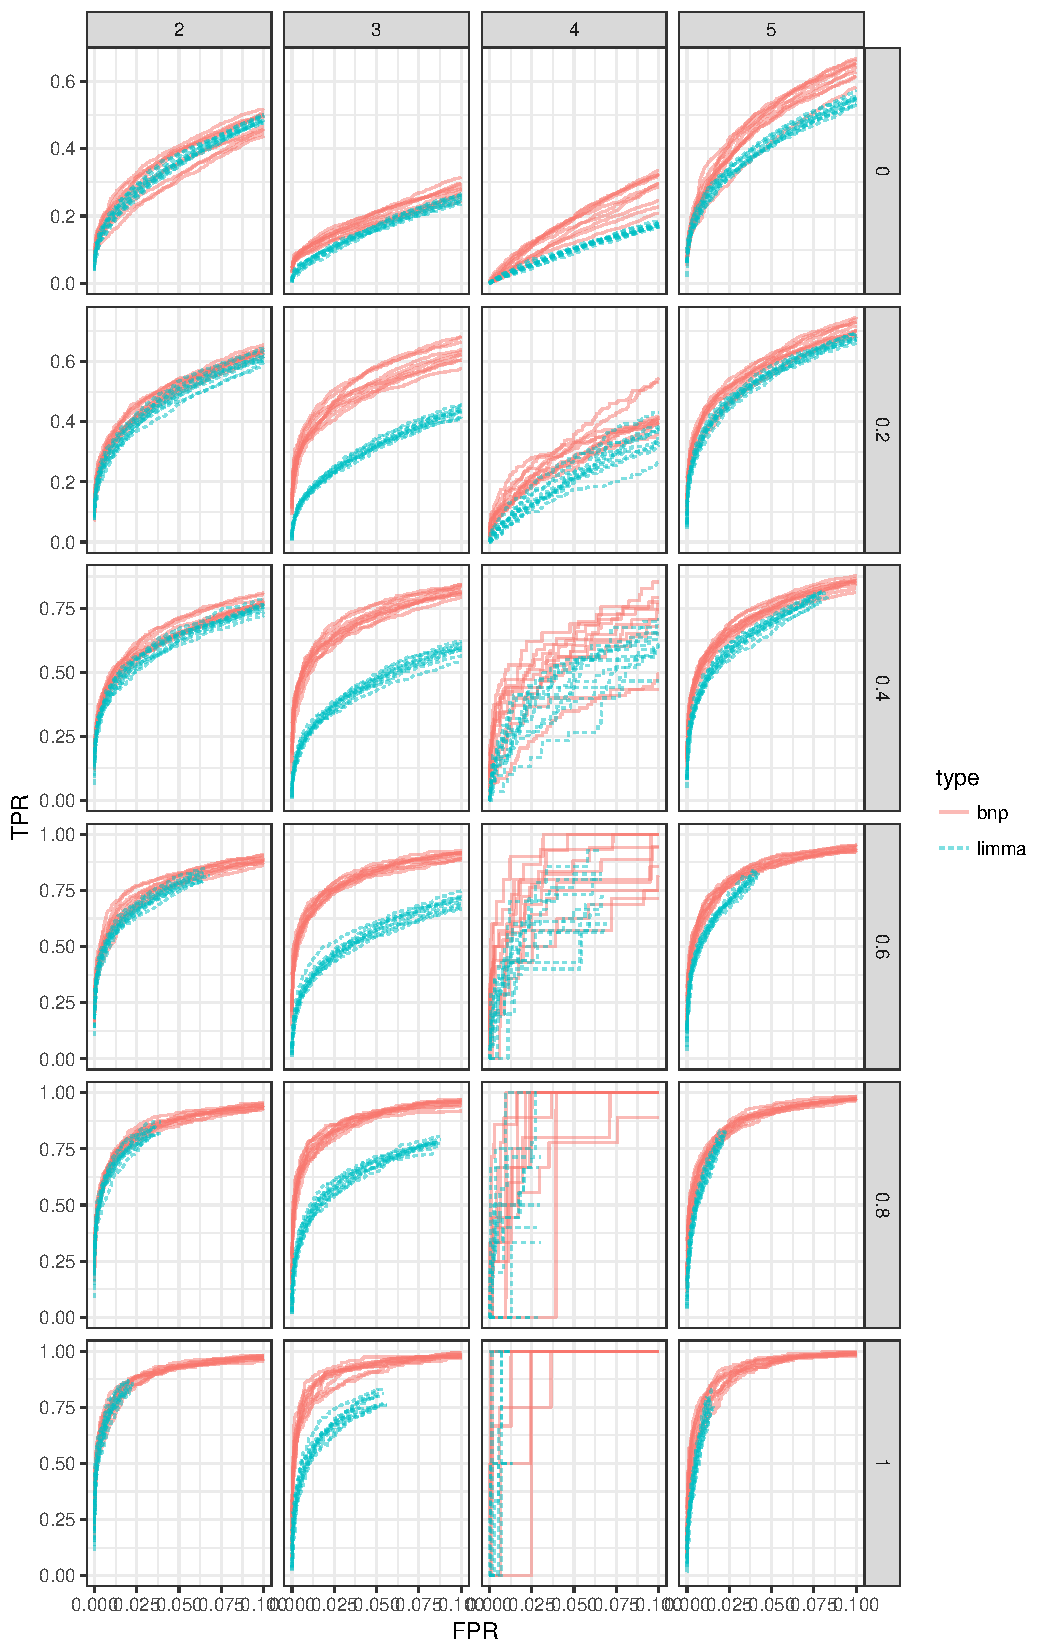
\includegraphics[width=.9\textwidth]{roc-ss1}
\label{roc-ss1}
\end{figure}

\section{Simulation study 2}
Much of the recent methods proposed for the analysis of RNA-seq data are based on an assumption that repeated sequencing of the same sample would produce Poisson distributed counts. For example, \cite{mccarthy} motivates the negative binomial model by showing that it has the right mean-variance relationship given the the above assumption and an assumption that the coefficient of variation is for constant within a gene. The favored approach is a negative binomial generalized linear model with log link function.

To compare estimation and accuracy of gene selection with existing methods designed for RNA-seq count data, we simulated count data by fitting the Paschold data with \texttt{voom/limma} and sampling a random subset of 10,000 genes without replacement. We then simulated normal data, conditioning on the estimates of $\beta_g$, $\sigma^2_g$, as well as the estimated precision weights. These simulated log-cpm values were then converted to log-counts, centering by $\log_2(\bar{R}_\cdot)-\log_2(10^6)$, where $\bar{R}_\cdot$ is the geometric mean of the estimated effective library sizes. Finally, these log-counts were exponentiated and rounded to obtain the simulated counts.

Simulation of counts:
To generate the simulated count data, we follow steps 1 and 2 of simulation study 1, and modify step 3: here, we bootstrap sample $W_{g,rep}$ from $W_g$ and simulate the pseudo-counts by
$$y^*_{g,rep} \sim N(X\beta_g,\sigma^2_gW_{g,rep}^{-1}).$$
Finally, we round $y^*_{g,rep}$ to obtain $y^*_{g,rep}$.




Generally: Generate count data, truth estimated from model, and compare voom pipelines.

Outputs: ROC curves, difference histograms

\section{Analysis of Paschold data}
To fit the Paschold data, we ran 4 chains, each for 40,000 iterations after 30,000 iterations of warmup. The samples were thinned by a factor of 40, for a total of 4,000 thinned post-warmup draws for each gene-specific parameter and $\alpha$. 



